
\section{Making a touch-instrument}

\subsection{Music}

\subsubsection{Notes}
A single tone $x$ has only two atributes: frequency $f_x$ and amplitude $a_x$ a.k.a. pitch and loudness . The wave of a note is a function of these two: $w_x(t) = a_x \cdot \sin( f_x \cdot t)$

In practice, a note will stop being played at some time. Therefore, the real function for a note would be $w_x(t) \cdot s(t_1, t_2)$, where $s$ is a step function. In FFT, however, we mostly treat a note as if it were a real periodic function - that is, never ending. We'll see details of this later. 

By the way: The same note played on a piano still sounds different from a violin because physical instruments never play one pure note. Instead, depending on the material, different overtones are played along with the basenote. 

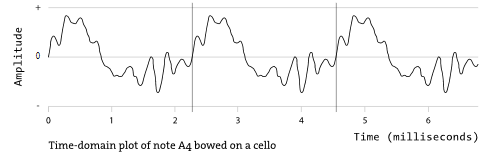
\includegraphics[width=10cm]{tdp.png}


\subsubsection{Harmony}
Instruments nowadays are tuned based on $a$, at 440 Hz. An octave higher would be $a'$ at 880 Hz. There are twelve steps from $a$ to $a'$, but their frequencies are not linearly, but exponentially spaced: 

\begin{itemize}
    \item linear: $f_x = \frac{12 + x}{12} f_a$
    \item exponential: $f_x = 2^{\frac{x}{12}} f_a$
\end{itemize}

Some combinations sound nice together:

\begin{itemize}
    \item Dur: {0,4,7}; $w(t) = w_a(t) + w_{cis}(t) + w_e(t)$
    \item Dur-Sept: {0,4,7,11}; $w(t) = w_a(t) + w_{cis}(t) + w_e(t) + w_{gis}(t)$
    \item Moll: {0,3,7}; $w(t) = w_a(t) + w_{c}(t) + w_e(t)$
    \item Moll-Sept: {}
\end{itemize}

They do sound nice together when the wave of their sum does display a nice pattern of peaks - that is, when the sum, too, displays a repeating pattern.

\subsubsection{Songs}

Several tones can be played together, thus adding up their waves: $w(t) = \sum_x w_x(t)$ Also, with every beat, new notes may be played. Thus for every beat a new analysis is required. 

\subsection{Deconstructing w(t) into fx and ax: the FFT}

The sound we hear in a song is really just a timeseries. Its values are the sum of the current amplitudes of all notes, i.o.w. it's just one single, complicated wave $w(t)$. The FFT takes that wave, chops it into windows of, say, a second, and tries to deconstruct the signal in each window into the original, simple waves $w_x(t)$ of the single notes $x$. 

So there are four steps to displaying a songs tones:

\begin{enumerate}
    \item Chop the signal into parts using the window-function (usually just a step-function). The window-function's length should be equal to the length of one beat.
    \item Take the first part and artificially elongate it by duplicating it over and over, thus creating a periodic signal.
    \item Do the FFT: represent this periodic signal as a sum of sines of different frequencies and amplitudes.
    \item Plot this.
    \item Repeat from step two with the next part of the choped-up signal.
\end{enumerate}

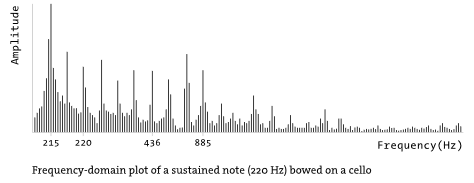
\includegraphics[width=10cm]{fdp.png}